\subsection{Data}\label{sec:data}

For this competition, we utilize two main components: a set of sequential decision making environments in Minecraft and a corresponding public large-scale dataset of human demonstrations. Through an online server which replicates these environments, we continue to engage the Minecraft community to add additional demonstrations to this dataset.

\subsubsection{Environment}

We define \emph{one primary competition environment}, \texttt{ObtainDiamond}, and six other auxiliary environments that encompass a significant portion of human Minecraft play. 
We select these environment domains to highlight many of the hardest challenges in reinforcement learning, such as sparse rewards, long reward horizons, and efficient hierarchical planning.


\paragraph{Primary Environment.}
As with last year's competition, the main task of this year's competition is solving the \texttt{Obtain} \texttt{Diamond} environment. 
In this environment, the agent begins in a random starting location without any items, and is tasked with obtaining a diamond. 
The agent receives a high reward for obtaining a diamond and smaller, auxiliary rewards for obtaining prerequisite items. 
Episodes end due to the agent dying, successfully obtaining a diamond, or reaching the maximum step count of 18000 frames (15 minutes).

\paragraph{Auxiliary Environments.}
%\begin{wrapfigure}{R}{0.5\textwidth}
\begin{figure}
    \begin{centering}
        \vspace{-10pt}
        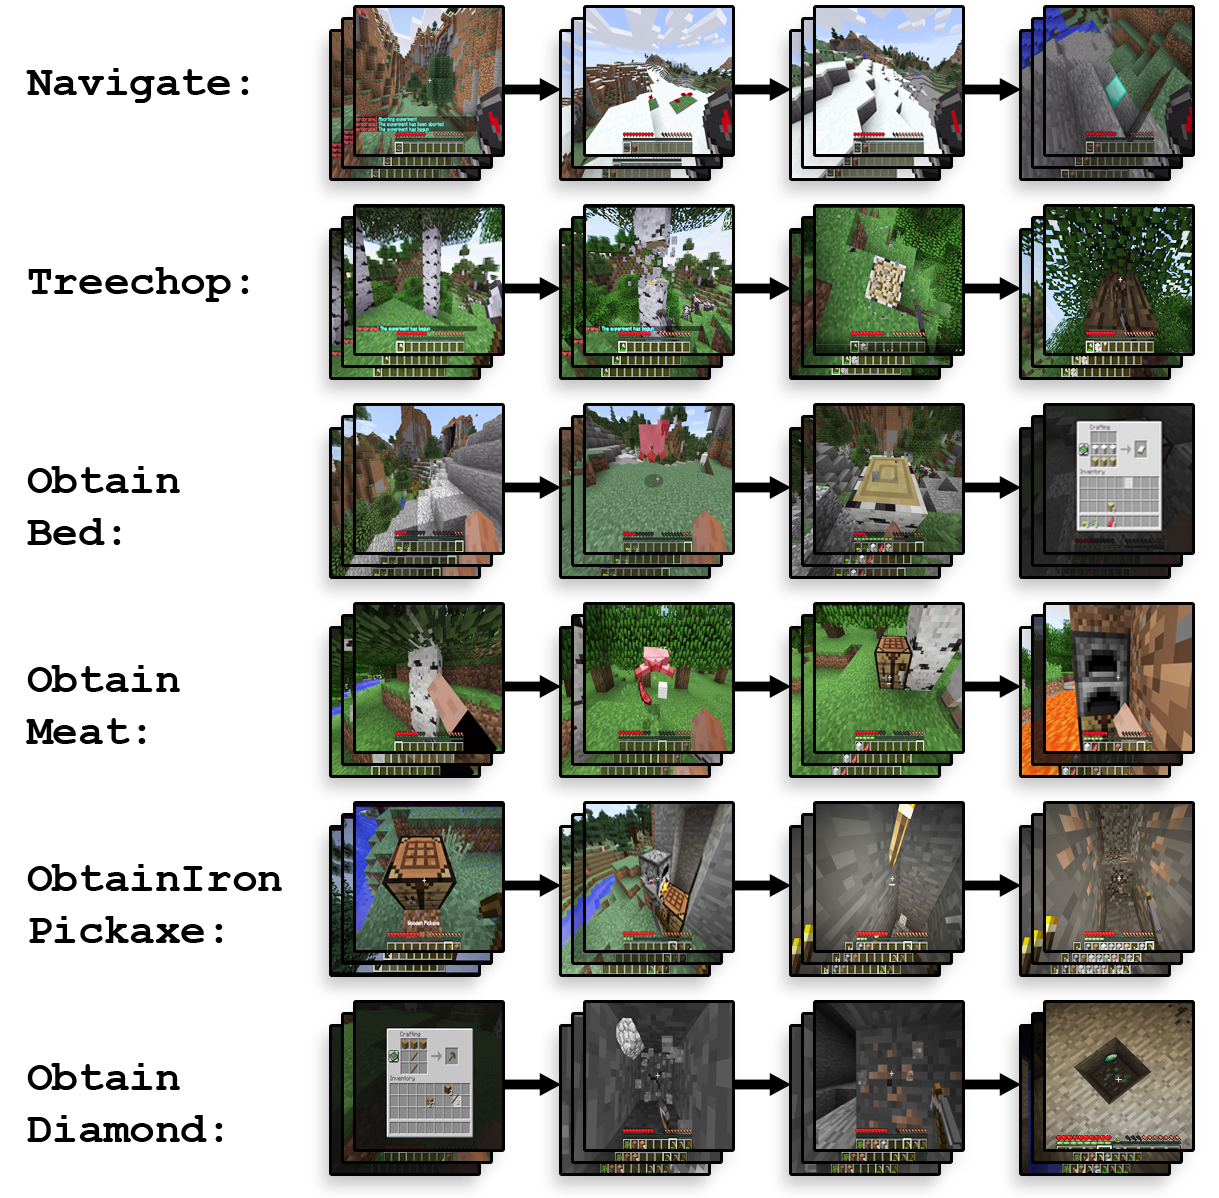
\includegraphics[width=0.49\textwidth]{./assets/tasks_smaller.png} 
        \caption{\small Images of various stages of six of seven total environments.}
        \label{fig:tasks}
        \vspace{-10pt}
    \end{centering}
    %\vspace{-10pt}
%\end{wrapfigure}
\end{figure}

The \texttt{ObtainDiamond} environment is a difficult environment; diamonds only exist in a small portion of the world and are 2-10 times rarer than other ores in Minecraft.
Furthermore, obtaining a diamond requires many prerequisite items. 
It is practically impossible for an agent to obtain a diamond via naive random exploration. 


We provide six auxiliary environments (in four families), which we believe will be useful for solving \texttt{ObtainDiamond}:
\begin{enumerate}
    \item \texttt{Navigate}: In this environment, the agent must move to a goal location, which represents a basic primitive used in many tasks in Minecraft. 
    In addition to standard observations, the agent has access to a ``compass'' observation,
    which points to a set location, 64 meters from the start location. 
    The agent is given a sparse reward (+100 upon reaching the goal, at which point the episode terminates). 
    We also support a dense, reward-shaped version of Navigate, in which the agent receives reward every tick corresponding to the change in distance between the agent and the goal.

    \item \texttt{Treechop}: In this environment, the agent must collect wood, a key resource in Minecraft and the first prerequisite item for diamonds.
    The agent begins in a forest biome (near many trees) with an iron axe for cutting trees. The agent is given +1 reward for obtaining each unit of wood, and the episode terminates once the agent obtains 64 units or the step limit is reached.
    
    \item \texttt{Obtain<Item>}:
    We include three additional obtain environments, similar to that of \texttt{ObtainDiamond},
    but with different goal items to obtain. They are:
    
\begin{enumerate}
    \item \texttt{CookedMeat}: cooked meat of a (cow, chicken, sheep, or pig), which is necessary for survival in Minecraft. In this environment, the agent is given a specific kind of meat to obtain.
    \item \texttt{Bed}: made out of dye, wool, and wood, an item that is also vital to Minecraft survival. In this environment, the agent is given a specific color of bed to create.
    \item \texttt{IronPickaxe}: is a final prerequisite item in obtaining a diamond.
    It is significantly easier to solve than \texttt{ObtainDiamond}: iron is
    20 times more common in the Minecraft world than diamonds, and this environment is typically solved by
    humans in less than 10 minutes.
\end{enumerate}

    \item \texttt{Survival}: This environment is the standard, open-ended game mode used by most human players when playing the game casually.
    There is no specified reward function, but data from this environment can be used
    to help train agents in more structured tasks, such as \texttt{ObtainDiamond}.

\end{enumerate}


\subsubsection{Dataset}

 \begin{figure}
    \begin{center}
        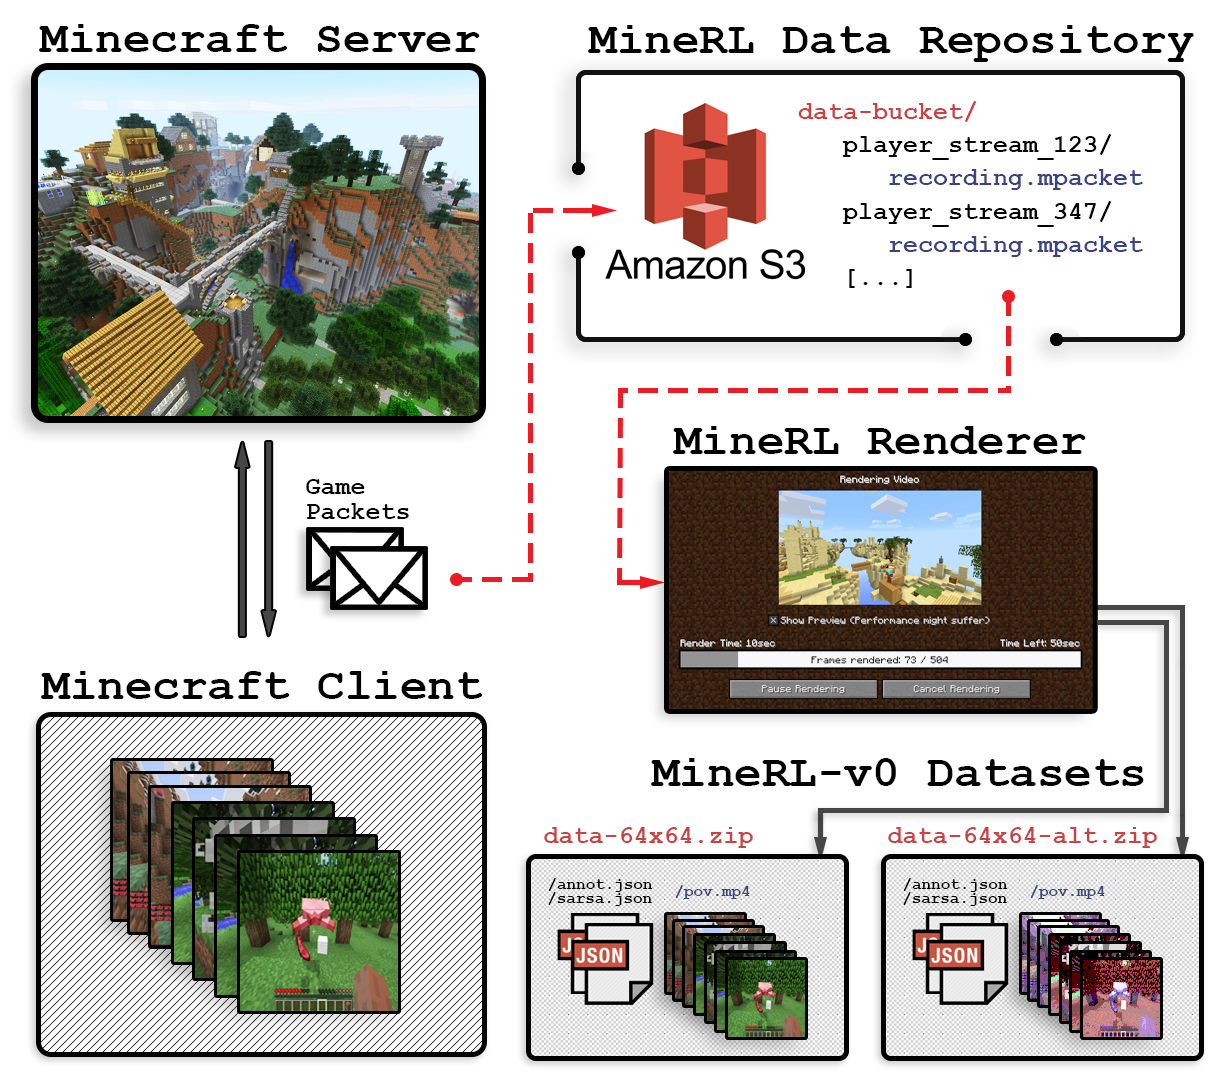
\includegraphics[width=0.47\textwidth]{./assets/datapipeline_new.png}
         \caption{\small A diagram of the MineRL data collection platform. Our
        system renders demonstrations from packet-level data, so we can
        easily rerender our data with different parameters.}
        \label{fig:platform_diagram}
    \end{center}
\end{figure}

The \minenet-v0 dataset consists of over 60 million state-action-(reward) tuples of recorded human demonstrations
over the seven environments mentioned above~\cite{gussminerlijcai2019}. In addition, we are actively working with the community to record additional human demonstrations. 
Trajectories are contiguously sampled every Minecraft game tick (at 20 game ticks per second). Each state is comprised of an RGB video frame of the player's point-of-view and a comprehensive set of features from the game-state at that tick:
player inventory, item collection events, distances to objectives, player attributes (health,
level, achievements), and details about the current GUI the player has open. The action
recorded at each tick consists of: all the keyboard presses, the change in view pitch and yaw
(mouse movements), player GUI interactions, and agglomerative
actions such as item crafting.

Accompanying the human trajectories are a large set of automatically generated annotations.
For all of the environments, we include metrics which indicate the quality of the demonstration, such as timestamped rewards, number of no-ops, number of deaths, and total score.
Additionally, trajectory meta-data includes timestamped markers for hierarchical labelings; e.g. when a house-like structure is built or certain objectives such as chopping down a tree are met. Data is made available both in the competition materials as well as through a standalone website\footnote{\url{http://minerl.io}}.

\subsubsection{Data Collection}
    In the previous MineRL competition, we used our novel platform for the collection of player trajectories in Minecraft, enabling the construction of the \minenet-v0 dataset.  In this second iteration of the competition, we will continue to utilize the platform with the hope of drastically expanding the existing dataset.
    As shown in Figure~\ref{fig:platform_diagram}, our platform consists of 
    (1) \emph{a public game server and website}, where we obtain permission to record trajectories of Minecraft players in natural gameplay;
    (2) \emph{a custom Minecraft client plugin}, which records all packet level communication between the client and the server, so we can re-simulate and re-render human demonstrations with modifications to the game state and graphics; 
    and (3) \emph{a data processing pipeline}, which enables us to produce automatically annotated datasets of task demonstrations.

    \paragraph{Data Acquisition.}
    Minecraft players find the \minenet~server on standard Minecraft server lists. 
        Players first use our webpage to provide IRB\footnote{The data collection study was approved by Carnegie Mellon University's institutional review board as \texttt{STUDY2018\_00000364}.} consent to have their gameplay anonymously recorded. Then, they download a plugin for their Minecraft client, which records and streams users' client-server game packets to the \minenet~data repository.
    When playing on our server, users select an environment to solve and receive in-game currency proportional to the amount of reward obtained. 
    For the \texttt{Survival} environment (where there is no known reward function), players
receive rewards only for duration of gameplay, so as not to impose an artificial reward function.


        
        
\paragraph{Data Pipeline.}
Our data pipeline allows us to resimulate recorded trajectories into several algorithmically consumable formats. 
    The pipeline serves as an extension to the core Minecraft game code and synchronously sends each recorded packet from the \minenet{} data repository to a Minecraft client using our custom API for automatic annotation and game-state modification. 
    This API allows us to add annotations based on any aspect of the game state accessible from existing Minecraft simulators. 
    Notably, it allows us to rerender the same data with different textures, shaders, and lighting-conditions which we use to create test and validation environment-dataset pairs for this competition.
 
\subsubsection{Data Usefulness}\label{sec:data_use}

\begin{wrapfigure}{r}{0.5\textwidth}

    \vspace{-25pt}
    \begin{center}
        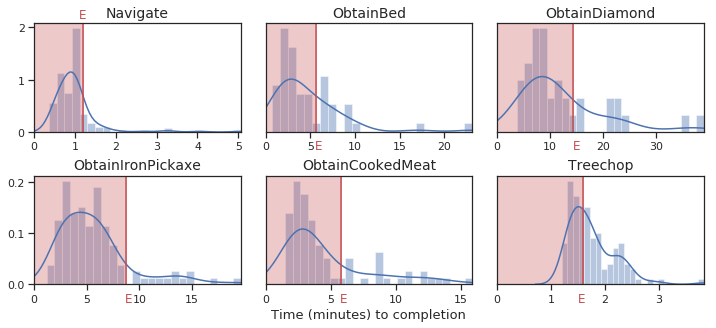
\includegraphics[width=0.49\textwidth]{./assets/task_performance.png}
    \caption{\small Normalized histograms of the lengths of human demonstration on various \minenet~tasks. The red {\color{red} \tiny\sf{E}} denotes the upper threshold  for expert play on each task.}
    \label{fig:human_quality}
    \end{center}
    \vspace{-20pt}
\end{wrapfigure}


\paragraph{Human Performance.}

    A majority of the human demonstrations in the dataset fall within the range of expert level play.
    Figure \ref{fig:human_quality} shows the distribution over trajectory length for each environment.
    The red region in each histogram denotes the range of times which correspond to play at an expert level, computed as the average time required for task completion by players with at least five years of Minecraft experience. 
    The large number of expert samples and rich labelings of demonstration 
    performance enable application of many standard imitation learning techniques which assume optimality of the base policy. 
    In addition, beginner and intermediate level trajectories 
    allow for the further development of techniques that leverage imperfect demonstrations.
    
    \begin{wrapfigure}{r}{0.5\textwidth}
        \begin{center}
            \vspace{-15pt}
            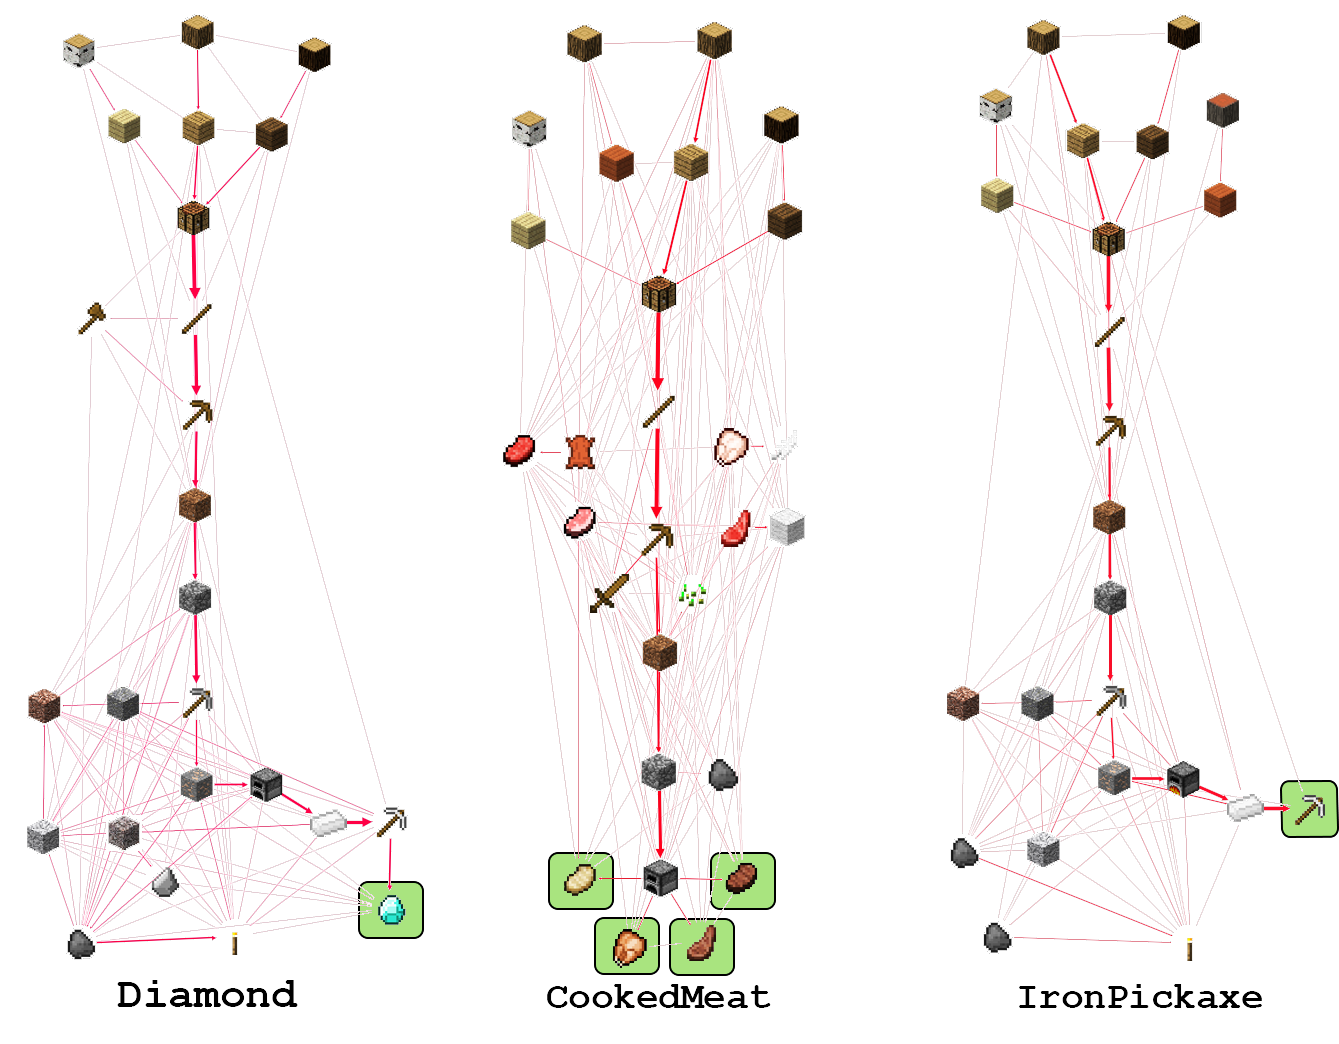
\includegraphics[width=0.47\textwidth]{./assets/item_graphs.png}
            \caption{\small Item precedence frequency graphs for \texttt{ObtainDiamond} (left), \texttt{ObtainCookedMeat} (middle), and \texttt{ObtainIronPickaxe} (right). The thickness of each line indicates the number of times a player collected item $A$ then subsequently item $B$. } \label{fig:task_hist}
            \vspace{-18pt}
        \end{center}
    \end{wrapfigure}
 

\paragraph{Hierarchality.} 

As shown in Figure~\ref{fig:hierarchicality}, Minecraft is deeply hierarchical, and the \minenet~data collection platform is designed to capture these hierarchies both explicitly and implicitly. 
Due to the subtask labelings provided in \minenet-v0, we can inspect and quantify the extent to which these environments overlap. 
Figure~\ref{fig:task_hist} shows precedence frequency graphs constructed from \minenet{} trajectories on the \texttt{ObtainDiamond}, \texttt{Obtain}\texttt{CookedMeat}, and \texttt{ObtainIronPickaxe} tasks.
In order to complete the \texttt{ObtainDiamond} task, an agent must complete the sub-goals of obtaining wood and stone, as well as constructing crafting tables and furnaces.
These subtasks also appear in \texttt{ObtainIronPickaxe} and \\ \texttt{ObtainCookedMeat}.
There is even greater overlap between \texttt{ObtainDiamond}
and \texttt{ObtainIronPickaxe}: most of the item hierarchy for \texttt{ObtainDiamond} consists of the hierarchy for \texttt{ObtainIronPickaxe}.


\paragraph{Interface}
Interacting with the environment and our data is as simple as a few lines of code.
Participants will be provided with an OpenAI Gym~\cite{gym} wrapper for the environment and a simple interface for loading demonstrations from the \minenet-v0 dataset as illustrated in Figure~\ref{fig:example_code}. 
Our data will be released in the form of Numpy \texttt{.npz} files composed of state-action-reward tuples in vector form,
and can be found along with accompanying documentation on the competition website.

\begin{figure}
    \centering
    \begin{subfigure}[b]{0.87\textwidth}
    \centering 
        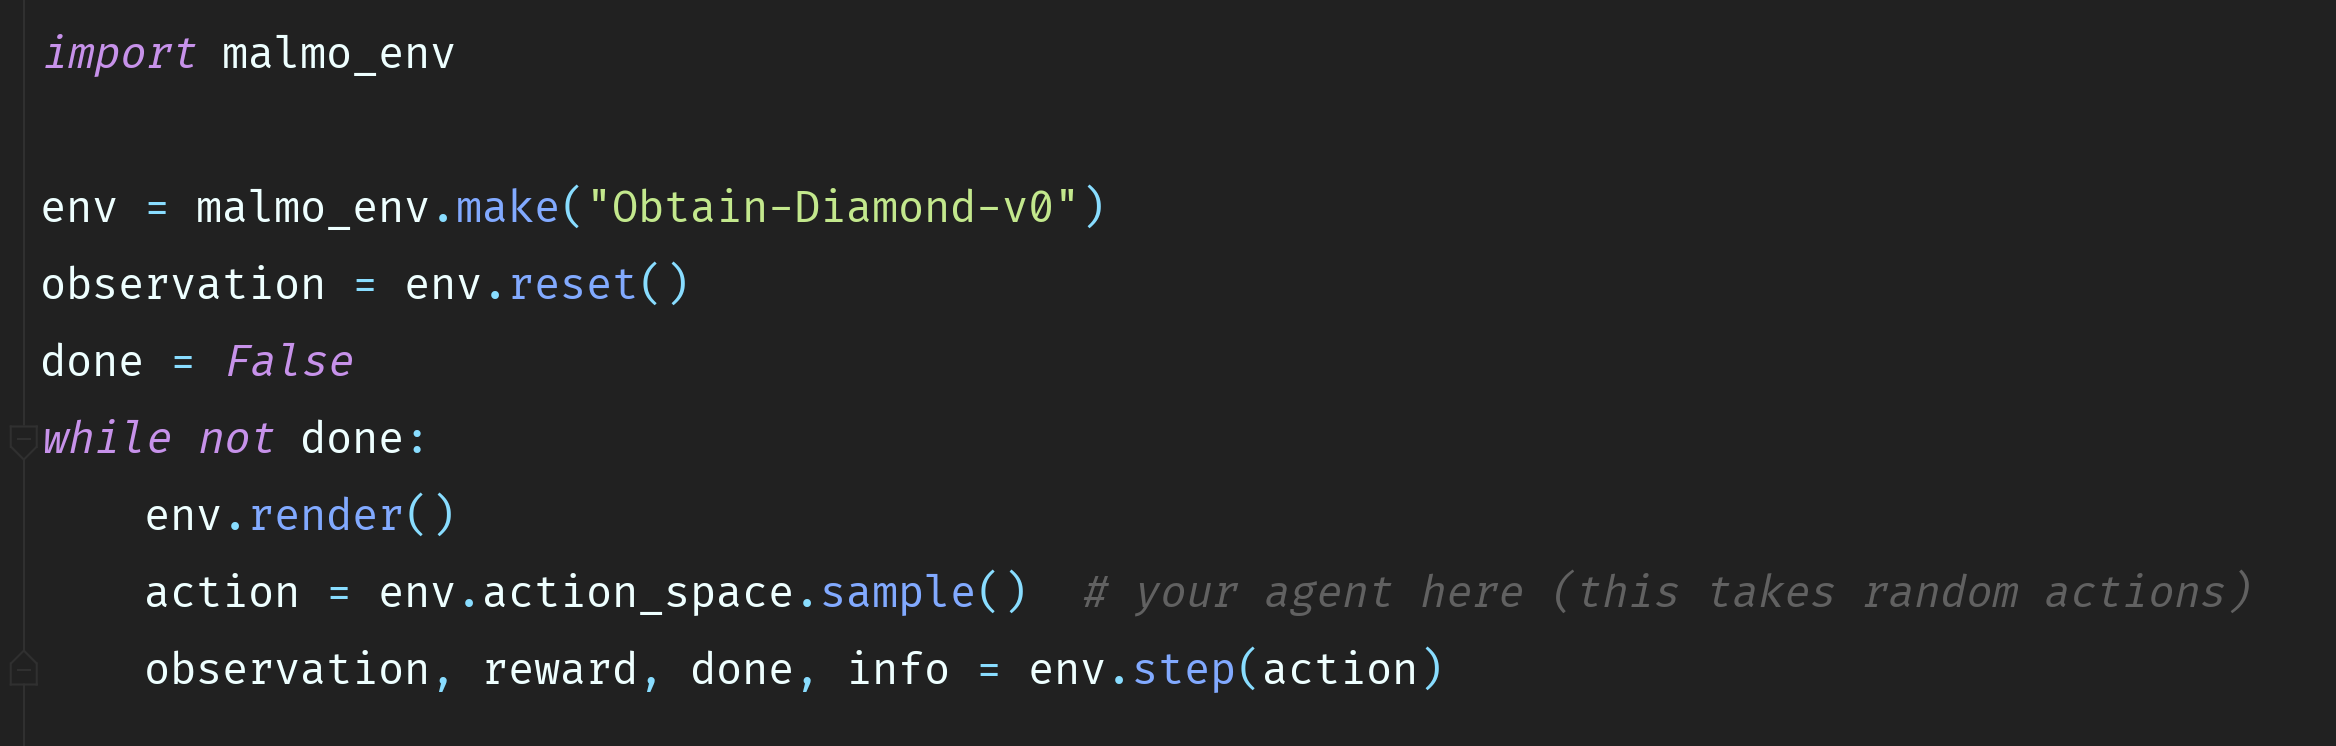
\includegraphics[width=0.87\textwidth]{./assets/malmo_env.png}
        \caption{\small Running a single episode of a random agent in \texttt{ObtainDiamond}. } 
        \label{fig:env_code}
    \end{subfigure}

    \begin{subfigure}[b]{0.87\textwidth}
    \centering
        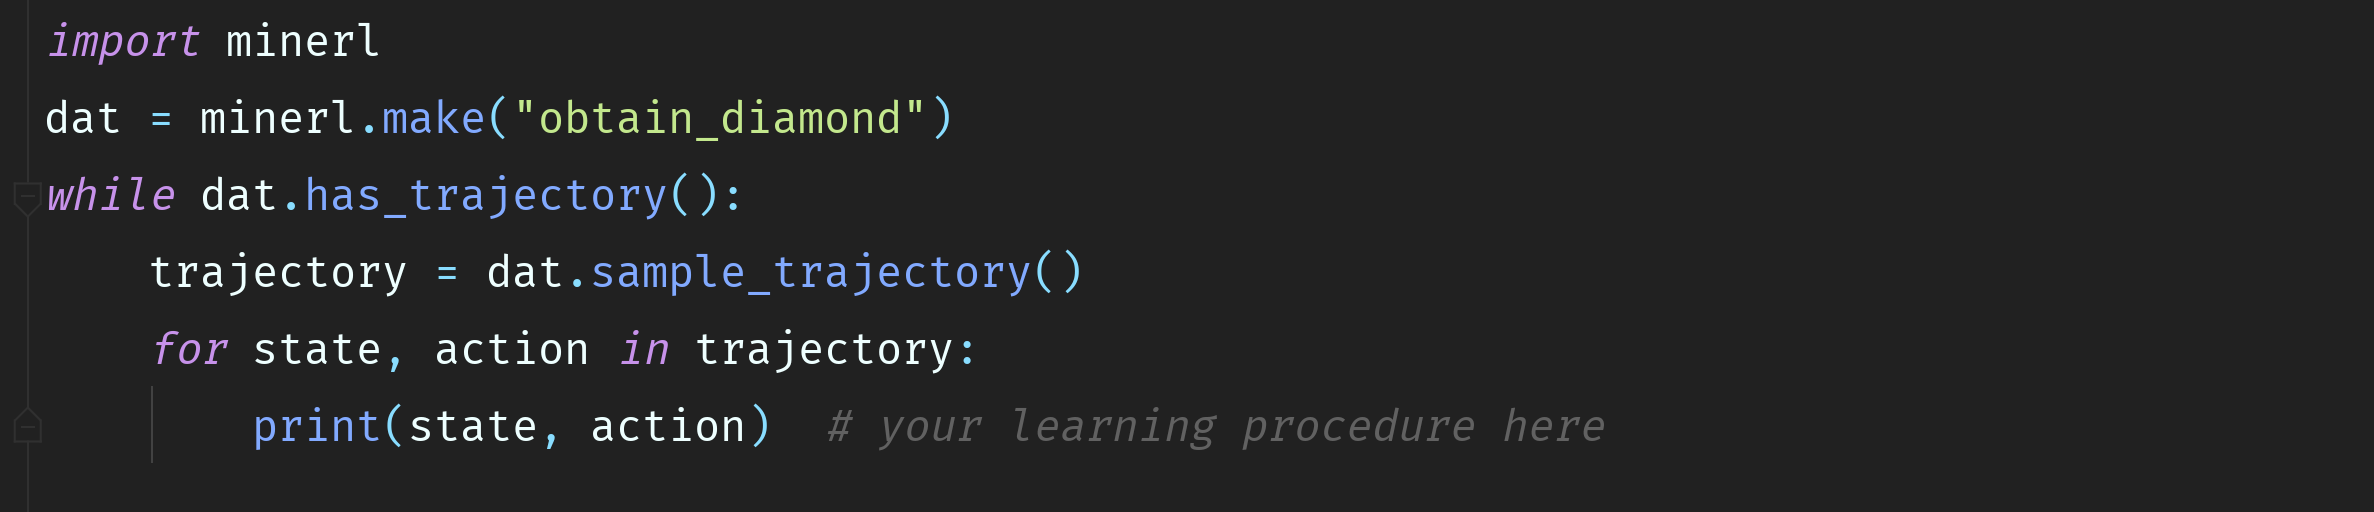
\includegraphics[width=0.87\textwidth]{./assets/mineral_dat_1.png}
        \caption{\small Utilizing individual trajectories of the \minenet dataset.} 
        \label{fig:mineral_code_1}
    \end{subfigure}

\begin{subfigure}[b]{0.87\textwidth}
    \centering
        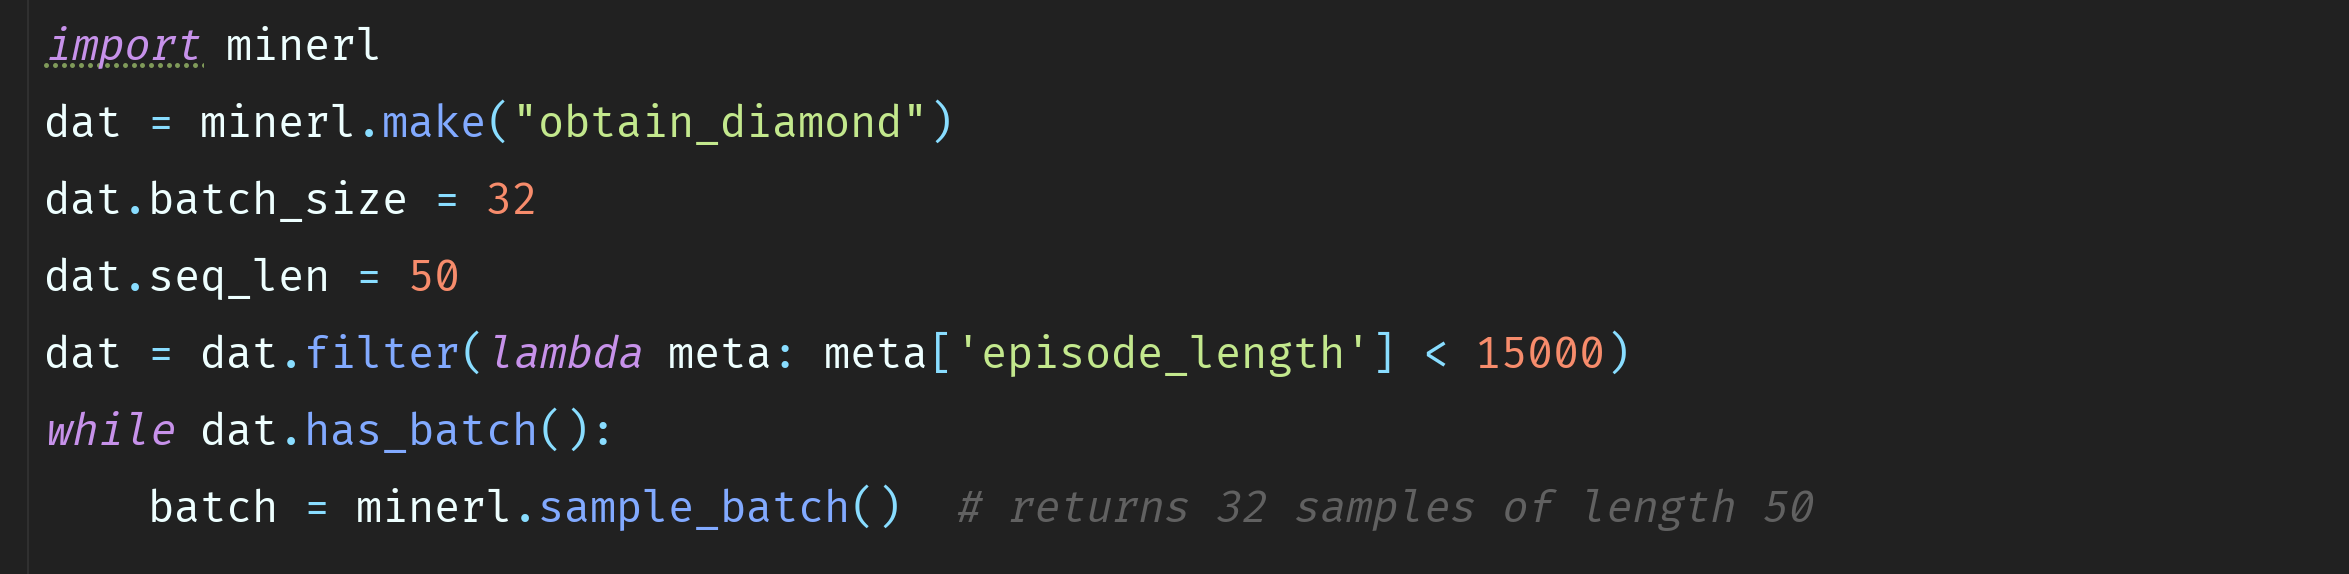
\includegraphics[width=0.87\textwidth]{./assets/mineral_dat_2.png}
        \caption{\small Using the \minenet  wrapper to filter demonstrations based on metadata} 
        \label{fig:mineral_code_2}
\end{subfigure}
\caption{\small Example code showing how to interact with MineRL data and environment.}
\label{fig:example_code}
\end{figure}

